\section{Introduction}

Exoskeletons are robotic interfaces for human-robot interaction where the highest physical symbiosis with the human operator is achieved.
Unlike many industrial robots  designed to exhibit a stiff structure and therefore to be used with a rigid position control, the exoskeletons are in direct contact with humans, so that  they have to satisfy  safety and compliance requirements.
In the last two decades, several exoskeleton solutions have been proposed using different implementation principles accordingly to the field of application.
Some important applications of the exoskeletons are post-stroke neurorehabilitation \cite{lo2012exoskeleton,pirondini2016evaluation}, assistance for limb movements, human power augmentation for lifting  heavy loads \cite{kim2016powered}) and teleoperation \cite{buongiorno2018wres, rebelo2014bilateral} to enhance the master immersivity and dexterity.
%
%Intro sulle architetture di giunto dove si illustrano le diverse tipologie, dove si contestualizza la nostra scelta e si motiva la nostra scelta.
\par In human-robot interaction devices, different actuation systems and technologies have been exploited.
Technologies based on geared solutions \cite{mihelj2007armin,vertechy2009development,carignan2005design}, tendon drives \cite{frisoli2009force,perry2007upper}, hybrid solutions (screw and cable actuators) \cite{garrec2008able} and  on pneumatic or hydraulic  actuation \cite{tsagarakis2003development,klein2010optimization} can be found in literature.
\par However in human-robot interaction applications, a fundamental characteristic of the actuation systems is its compliance. The actuators found in recent exoskeletons and humanoids can be classified accordingly to \cite{vanderborght2013variable} in two main categories, variable impedance actuators (VIA) and stiff actuators suitable for position control strategies. For HRI the use of purely position controlled solution is of limited interest. On the other hand, a variable impedance can be obtained by control (called active impedance by control) or can be a mechanical property, also defined passive impedance (inherent compliance or inherent damping). \figref{fig:exosActuators} shows a scheme of the two variable impedance typologies.
%
\par In inherent compliance systems an electric motor is coupled with a spring with fixed (Series Elastic Actuator - SEA) or variable stiffness (Variable Stiffness Actuators – VSA). Inherent damping systems are based on the control of the friction by means of eddy currents, controlled rheology or fluid dynamic. Recently double actuation architectures have been developed for variable impedance actuators	\cite{tagliamonte2012double}, coupling the stiff motor in parallel with the elastic element (Parallel Elastic Actuators - PEA).  Both SEA and VSA have been implemented in exoskeleton as for example in Lopes \cite{veneman2007design}, an exoskeleton for the gait assistance that is based on SEA actuation, or in NEUROexos elbow exoskeleton \cite{vitiello2013neuroexos} that is based on VSA and in ALTACRO locomotion exoskeleton \cite{cherelle2010maccepa} that introduces a Mechanically Adjustable Compliance and Controllable Equilibrium Position Actuator (MACCEPA).
%. 
\par All the variable impedance actuators have the advantage of absorbing impacts and SEA, PEA and VSA (inherent compliance) can eventually mechanically storage energy during passive phases and release it in active phases of the movement cycle. In general, adding a series elastic element reduces the peak power demand on the motor.  VSAs generally use two motors which increases the size, weight and complexity of the actuator in comparison with an SEA \cite{wolf2011dlr}.

\par On the other side, active impedance systems are electric motors coupled with a transmission/reduction system; they can be classified
according to the backdrivability and sensing system. Force controlled actuators implement a force/torque sensor
in the joint and can achieve impedance behavior by closed-loop control.
In general traditional actuators, due to the absence of elastic or damping elements, can be lighter and more compact
than passive variable impedance actuators, but their time response and dynamic bandwidth is limited by control and electrical properties of actuators, such as maximum velocity of electrical motor.
%
%The actuation system influences the control design: active exoskeletons can be classified as impedance based design (open-loop impedance control \cite{frisoli2009force} and impedance control with force feedback) or admittance-based design (admittance control with position feedback) \cite{carignan2000closed}.
%
%Open-loop impedance control exoskeletons rely on lightweight designs with joint-delocated motors and backdrivable mechanical solutions, typically implemented making use of tendon transmissions \cite{frisoli2009force}, \cite{perry2007upper}; the most challenging limitations are the friction effects due to the transmission system, that can be compensated only by means of feed-forward compensation based on approximate models, the complexity of the transmission and the difficulty to be mechanically configured in a bilateral configuration, working both for left and right arm. 
%On the other side admittance-based design requires force sensing and can achieve higher stiffness values, but relies on the adopted control for canceling system dynamics and inertia.
%Exoskeleton with a single force/torque sensor localization, such as one torque sensor at the exoskeleton elbow joint and a six-axis force/torque sensor at the exoskeleton handle \cite{carignan2008controlling} or shoulder \cite{nef2007armin}, can accurately regulate interaction forces at the exoskeleton terminal link (i.e. the handle) only.
%Lightweight robots with joint torque sensors \cite{albu2007dlr} allow for multi-contact force/torque control (i.e. the regulation of interaction force/torques at multiple points distributed over multiple links).
%
%
%The correct estimation of interaction force between human and exoskeleton in admittance designs requires control approaches that compensate for friction, inertial and gravity properties of the exoskeleton mechanical structure, but  a complete cancellation of these effects is  difficult to achieve.
%
\begin{figure}[]
	\centering
	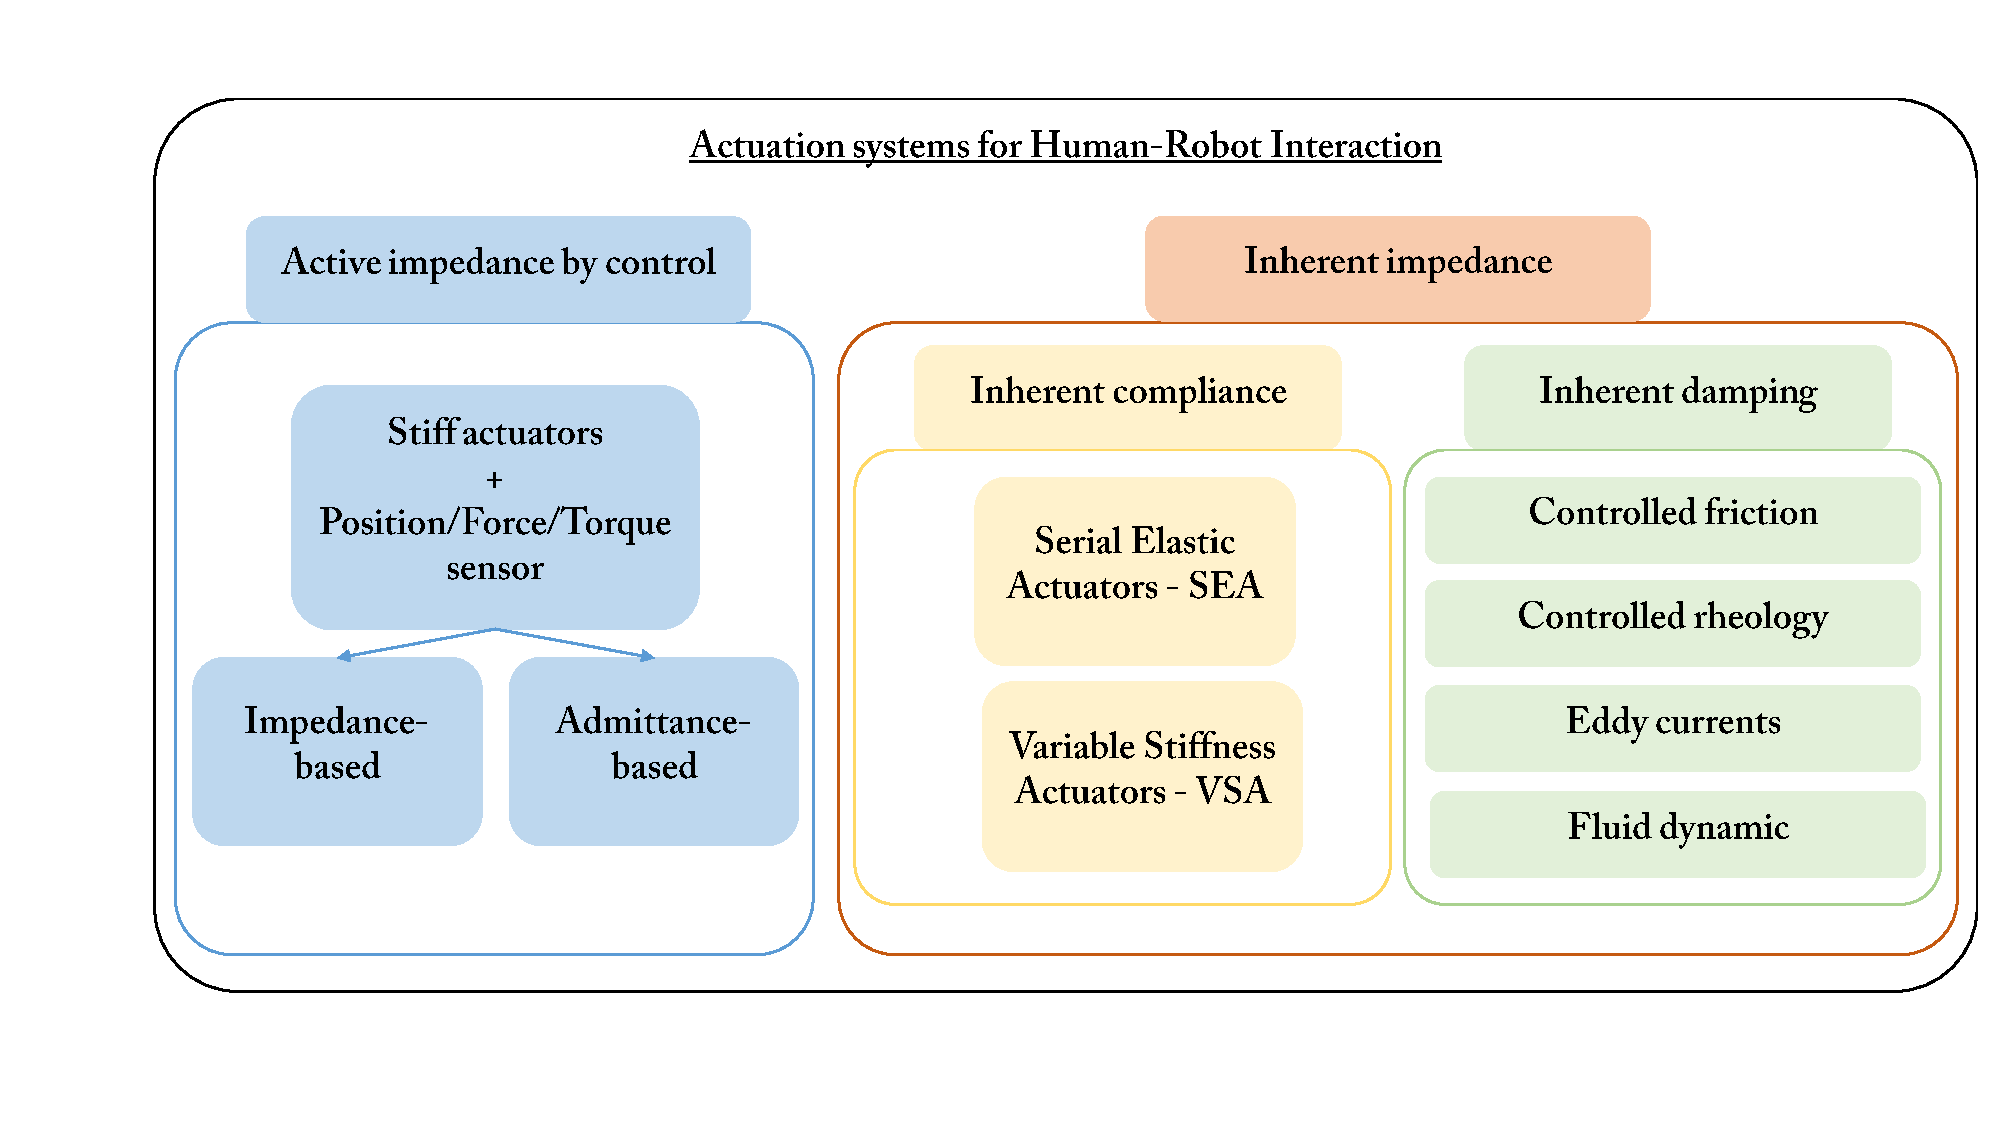
\includegraphics[width=1 \columnwidth]{actuators}
	\caption{Schema of variable impedance actuation systems for human-robot interaction. The impedance can be simulated and  actively changed by control (this relies on position and torque sensors) or can be an inherent mechanical property of the actuator. In the latter case the mechanical stiffness can be a fixed value (SEA) or can be adjusted (VSA), and the damping can be controlled.}
	\label{fig:exosActuators}
\end{figure}
%
\begin{figure}[htb]
	\centering
	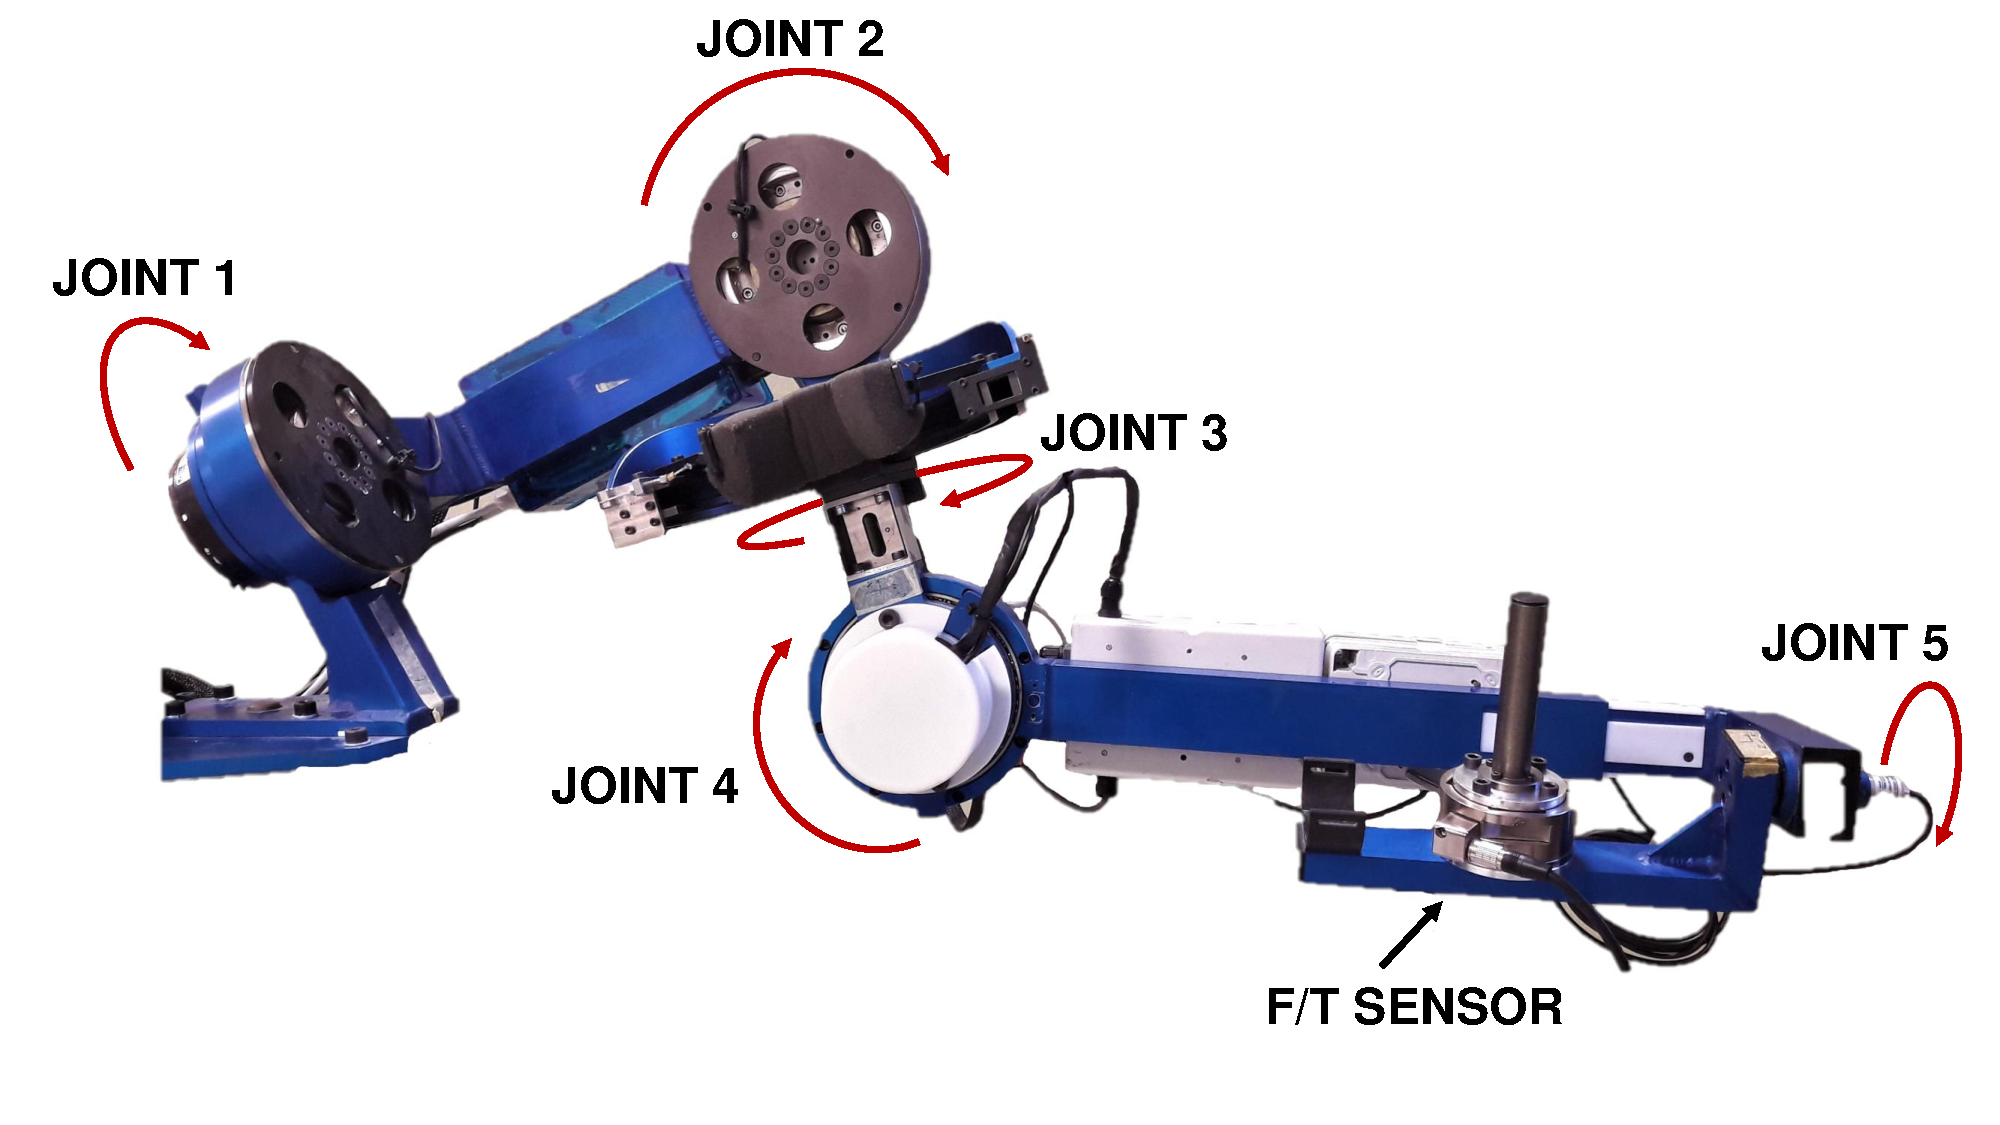
\includegraphics[width=0.95\columnwidth]{RehabDescription} 
	\caption{The Rehab-Exos. It is a 5 DOF upper-limb exoskeleton  with 4 actuated joints. The joints $J_1$, $J_2$ and $J_4$ share the same characteristics: high reduction ratio (100:1) by means of harmonic drive, embedded torque sensor and maximum actuation torque of 150 \ Nm. The joint $J_3$ is composed by a semi-circular guide actuated by a DC motor through tendon transmission. Joint $J_5$ is passive and the exoskeleton is equipped of a force/torque sensor at the end-effector that is used for evaluation purposes.}
	\label{fig:rehabexos1} 
\end{figure}
%
\par Solutions based on joint torque sensor have been proposed in the last years mostly for lower limb exoskeletons. In \cite{kim2015design} and in \cite{aguirre2011design} two knee exoskeletons based on joint torque sensor were presented; the latter exoskeleton implements an admittance control based on the torque sensor reads. In \cite{hwang2015method} the torque sensor for a lower limb exoskeleton allows to accurately estimate the human muscular torque that were exerted during the human-robot interaction. The advantage of joint torque sensor based solutions is their compactness and robustness, but when the torque sensor is embedded in the joint it is sensitive to the link inertia in addition to the human interaction torques, thus affecting the system transparency. A mechanical solution is presented in \cite{zanotto2013improving} where the transparency of a lower-limb exoskeleton has been improved by positioning the force/torque sensor on the supporting cuffs, that is at the interaction point between the human leg and the exoskeleton.
\par Even if SEA and VSA are less compact then traditional actuators, for example \cite{cestari2014ares} proposed a solution based on a VSA for an exoskeleton of the leg that reduced the lateral size and integrates a torque sensor based on spring's deflection reads. Sensors used to measure these deflections are generally encoders \cite{dos2017design} and potentiometers \cite{junior2016series}; the latter usually require custom mechanical supports to avoid errors related with its sensitivity to misalignments.
While the deflection based force estimation becomes a most widely utilized method for the SEAs and VSAs and performs fidelity force control performance in various robotic applications, there are still difficulties because of the practical issues such as spring deflection measurement error or noise of the encoder signal \cite{lee2018integrated}. These factors have much negative impact on SEA with high stiffness. In \cite{leal2018polymer}, for example, a polymer optical fiber has been mounted on the torsional spring of a SEA to read angles and torques in a more accurate way without considerably enlarging the size of the actuator at the cost of a more specific system electronics.
\par Thus, the use of inherent compliant actuation systems rather than achieving compliance by control systems is not a trivial choice and it depends on the desired mechanical features and is the result of a trade-off among compactness, weight, simplicity, costs, safety, efficiency and compliance.
A good trade-off that prefer compactness, simplicity and uses just one motor is an active impedance by control actuation system that integrates an elastic component to transmit and to measure axial torques at the same time.

\par In this paper we address the issue of a collaborative robot behavior, by designing an upper limb exoskeleton based on joint torque actuators endowing joint torque sensors and extend our previously work presented in \cite{solazzi2014interaction}. 
The Rehab-Exos allows to obtain a physical interaction characterized by good transparency and force rendering accuracy, it is capable to exert a wide range of forces and at the same time it exhibits high position accuracy due to high gear reduction ratio.
\par The first part of the paper widely treats the critical issue due to the use of a torque sensor embedded in the joint and in particular the sensitivity to non-axial load has been studied. Then, in the second part the joint model and the control technique are presented.
\par In particular, for what concern transparency we propose an interaction torque control that take into account the multi-dof non linear system dynamics and provide a compensation of non-linear effects such as inertial and gravity components, to achieve an accurate estimation of human interaction force.
This is accomplished by a single joint optimum observer that ensures joint torque tracking, while a centralized control estimates and compensates for the dynamics of the whole system. Moreover, we have evaluated the effect of dynamic compensation on system transparency highlighting good results.
\par To validate the proposed control as well as the chosen mechanical architecture, the full-state feedback control  has been compared with a basic feedback control and a passivity-based feedback control in two tasks: the zero desired force and the contact with a virtual stiff flat surface. 
For what concern haptic rendering, we evaluate at geometrical level the quantitative and qualitative behavior of the proposed controller and we compared it with the other two implemented controllers.
Results reward the chosen mechanical and control strategy as presented in the last part of this paper.
 
\par This paper is structured as follows: Section \ref{sec:systemDesign} presents the design of the Rehab-Exos with a particular focus on the strain gauge-based torque sensor design and issues. Section \ref{Single joint model} provides a mathematical model of the single joint whereas in the Section \ref{Full dynamics model} the full dynamics model of the Rehab-Exos is described. Section \ref{sec:Full_state_feedback_controllers} explains the proposed full state feedback controller and recalls two torque controls already known in literature. Section \ref{sec:experimentsResults} presents the experiments and the obtained results.
Finally, discussions and conclusions are addressed in Sections \ref{sec:discussion} and \ref{sec:conclusion} respectively.  

%
%Active exoskeleton systems are robotic devices that can be worn on the user's body, implying that they should satisfy requirements of safety and better compliance.
%After the Fukushima event in Japan, the application of these human-robot interfaces in the area of rescue robotics and teleoperation has became an emerging field of research,
%for which the development of upper limb active exoskeletons with dexterous manipulation abilities has become a hot topic of research.
%Another relevant sector of application of active exoskeletons is represented by neuro-motor rehabilitation post-stroke \cite{lo2012exoskeleton}, where different prototypes and commercial solutions have been recently proposed.
%
%
%While the general rationale for the design of high performance haptic interfaces are the satisfaction of the requirements of high force fidelity, transparency
%and backdrivability, specific issues need to be addressed in exoskeleton design in terms of safety, kinematics and ....
%
%For what concerns, upper limb exoskeletons, we should consider:
%\begin{description}
%\item[User requirements] Safety: the structure is always in close contact with the user
%\item[Design issues, kinematics, mechanical design]
%The kinematics should be adjusted to user arm, Possibility of adjusting the size of the system to avoid internal forces
%Complexity of shoulder motion, Non periodicity of upper limb movement compared to lower limb, Intrinsic 3D spatial motion Both left and right arm schemes should be implementable
%\item[Design issues, control] Low inertia should be achieved, possibility of employing force sensors, Remote vs. local actuation, High forces required (no gravity cancellation provided by support elements e.g., support plans)
%\end{description}
%
%%In SSSA there is a consolidated experience in the design and development of new exoskeleton systems \cite{frisoli2005new}, as shown in figure~\ref{fig:exos@SSSA}.
%
%%%%%%%%%%%%%%%%%%%%%%%%%%%%%%%%%%%%%%%%%%%%%%%%%%%%%%%%%%%%%%%%%%%%%%%%%%%%%%%%%%%%%%%%%%%%%%%%%%%%%%%%%%%%%%%%%%%%
%%%%%%%%%%%%%%%%%%%%%%%%%%%%%%%%%%%%%%%%%%%%%%%%%%%%%%%%%%%%%%%%%%%%%%%%%%%%%%%%%%%%%%%%%%%%%%%%%%%%%%%%%%%%%%%%%%%%
%%%%%%%%%%%%%%%%%%%%%%%%%%%%%%%%%%%%%%%%%%%%%%%%%%%%%%%%%%%%%%%%%%%%%%%%%%%%%%%%%%%%%%%%%%%%%%%%%%%%%%%%%%%%%%%%%%%%
%%%%%%%%%%%%%%%%%%%%%%%%%%%%%%%%%%%%%%%%%%%%%%%%%%%%%%%%%%%%%%%%%%%%%%%%%%%%%%%%%%%%%%%%%%%%%%%%%%%%%%%%%%%%%%%%%%%%
